\documentclass{beamer}
\usetheme{default} 

\setbeamercolor{structure}{fg=green!40!black} 
\usebackgroundtemplate{
    \centering
\includegraphics[width=\paperwidth,height=\paperheight]{images/android_wall}
}
\setbeamertemplate{navigation symbols}{}

\usepackage[polish]{babel}
\usepackage[utf8x]{inputenc}
\usepackage{t1enc}
\usepackage{default}
\usepackage{listings}

\lstset{language=java, basicstyle=\small, commentstyle=\color{gray}}
\lstset{frame=single}

\usefoottemplate{
  \vbox{
    \tinycolouredline{structure!25}{
      \color{black}\textbf{	
        \insertshortauthor\hfill
        Android @ Szczecin 2011
      } 
    }
%    \tinycolouredline{structure}{
%      \color{white}\textbf{\insertshorttitle}\hfill
%    } 
  }
}

\title{Android @ Szczecin \\ 2011}
\author{Konrad Malawski \\ konrad.malawski@java.pl}

\begin{document}


\begin{frame}
 \begin{center}
  \Huge{AppWidgets}
 \end{center}
\end{frame}

\begin{frame}\frametitle{AppWidget}
\begin{itemize}
 \item Good news: Bardzo proste!
 \item AppWidget = specjalny BroadcastReciever
 \item a rozmiar etc, deklarujemy w \textbf{res/xml/my\_widget.xml}
\end{itemize}
\end{frame}


\begin{frame}[fragile]\frametitle{AppWidgetProvider}
\textbf{AppWidgetProvider}, musi zostać zarejestrowany w \textbf{AndroidManifest.xml} (w <application/>):
\begin{lstlisting}
<receiver android:name=".ui.appwidgets.MyWidgetProvider">
  <intent-filter>
    <action android:name="android.appwidget.action.APPWIDGET_UPDATE"/>
  </intent-filter>
  <meta-data android:name="android.appwidget.provider"
             android:resource="@xml/my_widget"/>
</receiver>
\end{lstlisting}
\end{frame}

\begin{frame}[fragile]\frametitle{res/xml/\textbf{my\_widget.xml}}
\begin{lstlisting}
<appwidget-provider xmlns:android="http://schemas.android.com/apk/res/android"
    android:minWidth="294dp"
    android:minHeight="72dp"
    android:updatePeriodMillis="86400000"
    android:previewImage="@drawable/preview_widget"
    android:initialLayout="@layout/widget">
</appwidget-provider>
\end{lstlisting}
Deklarowanie tego w XML jest wygodniejsze - mamy filtrowanie folderów (-v11).
\end{frame}



\begin{frame}[fragile]\frametitle{AppWidget - implementacja}
\begin{lstlisting}
public class MyWidgetProvider extends AppWidgetProvider {

  @Override
  public void onUpdate(Context context, 
                       AppWidgetManager appWidgetManager, 
                       int[] appWidgetIds) {

    // Provider obsluguje WIELE (N) widzetow!
    final int N = appWidgetIds.length;

    // aktualizujemy kazgego
    for (int i = 0; i < N; i++) {
      int appWidgetId = appWidgetIds[i];
      populateView(context, appWidgetManager, 
                            appWidgetId);
    }
  }
\end{lstlisting}
\end{frame}

\begin{frame}[fragile]\frametitle{AppWidget - implementacja}
\begin{lstlisting}
private void populateView(Context context, AppWidgetManager appWidgetManager, int appWidgetId) {
  // Przygotowujemy intent do odpalenia "on click"
  Intent intent = new Intent(context, ViewDetailsActivity.class);
  PendingIntent pendingIntent = PendingIntent.getActivity(context, 0, intent, 0);

  // rejestrujemy onClickListener'a troszke inaczej:
  RemoteViews views = new RemoteViews(context.getPackageName(), R.layout.widget);
  views.setOnClickPendingIntent(R.id.container, pendingIntent);
 
  // aktualizujemy widok widzetu (prosimy menagera o to)
  appWidgetManager.updateAppWidget(appWidgetId, views);
}
} // end of class
\end{lstlisting}
\end{frame}



\begin{frame}
\begin{center}
\Huge{Notifications}
\end{center}
\end{frame}

\begin{frame}\frametitle{Notificaion - przykład}
\begin{figure}
 \centering
 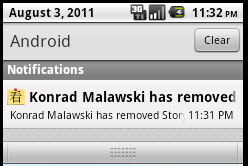
\includegraphics[width=0.7\textwidth]{images/notification_android_2_2}
\end{figure}
\end{frame}


\begin{frame}[fragile]\frametitle{NorificationManager}
\begin{lstlisting}
class MyActivity extends RoboActivity {
  
  @Inject
  NotificationManager notificationManager;

}
\end{lstlisting}
\pause Albo oczywiście \textbf{Service}.
\end{frame}


\begin{frame}[fragile]\frametitle{NorificationManager - 1/3}
\begin{lstlisting}
int icon = R.drawable.ic_kanbanery;
long when = System.currentTimeMillis();

Notification notification = new Notification(icon, title, when);

// ...
\end{lstlisting}
\end{frame}


\begin{frame}[fragile]\frametitle{NorificationManager - 2/3}
\begin{lstlisting}
int icon = R.drawable.ic_kanbanery;
long when = System.currentTimeMillis();

Notification notification = new Notification(icon, title, when);

Intent notificationIntent = new Intent(this, ColumnsActivity.class);
PendingIntent onClickIntent = PendingIntent.getActivity(this, 0, notificationIntent, 0);

// ...
\end{lstlisting}
\end{frame}

\begin{frame}[fragile]\frametitle{NotificationManager - 3/3}
\begin{lstlisting}
int icon = R.drawable.ic_kanbanery;
long when = System.currentTimeMillis();

Notification notification = 
                 new Notification(icon, title, when);

Intent notificationIntent = new Intent(this, 
                              ColumnsActivity.class);
PendingIntent contentIntent = PendingIntent
        .getActivity(this, 0, notificationIntent, 0);

notification.setLatestEventInfo(context, title, 
                                msg, contentIntent);
notification.flags = Notification.FLAG_AUTO_CANCEL;


notificationManager.notify(ACTION_ID, // explain 
                           notification);
\end{lstlisting}
\end{frame}


\begin{frame}
\begin{center}
 \Huge{Service}
\end{center}
\end{frame}

\begin{frame}\frametitle{Service}
\begin{itemize}
 \item Service uruchamiany jest na tym samym głównym wątku co Activity (UIThread)
 \pause \item Oczywiście nie wolno mu go ,,zablokować''
 \pause \item Service działa ,,w tle'', nie ma UI
 \pause \item Service to \textbf{NIE} osobny proces
 \pause \item Service to \textbf{NIE} osobny wątek
 \pause \item Kontunuuje działanie nawet po zamknięciu wszelkich Activity aplikacji
\end{itemize}
\end{frame}

\begin{frame}\frametitle{2 ,,rodzaje'' Service (choć ta sama klasa)}
Mimo, że zawsze mówimy o \textbf{android.app.Service}, możemy mieć na myśli 2 ,,typy'' Service:
\begin{itemize}
 \pause \item ,,\textbf{Uruchamiany}'' celem zrobienia czegoś przez nas - \textbf{startService(Intent)}
 \pause \item ,,\textbf{Udostępniany}'' celem udostępnienia komuś API, nawet zewnętrznym aplikacjom! - tutaj mowa o \textbf{IBinder} i \textbf{onBind()}. (Bardzo zaawansowane rzeczy można tutaj robić, vide AIDL)
\end{itemize}
\pause Nas interesuje jedynie pierwszy rodzaj serwisu.
\end{frame}

\begin{frame}\frametitle{Service lifecycle}
 \begin{itemize}
  \item \textbf{onCreate()} - gdy jeszcze nie był utworzony, a zawołano \textbf{startService()}
  \pause \item \textbf{onStart()} - przy uruchomieniu Serwisu, po onCreate() - tutaj umieszczamy ,,logikę''
  \pause \item \textbf{onBind()} - w przypadku ,,uruchomienia'' przez \textbf{bindService()}, na razie nas nie interesuje - możemy zwracać \textbf{null}
  \pause \item \textbf{onStartCommand()} - wołany za każdym radem gdy ktoś startuje service. \textit{OnCreate() nie zostałby zawołany jak 2 razy pod rząd zastartujesz serwis!}
  \pause \item \textbf{onDestroy()} - wiadomo, gdy servis zostaje zatrzymywany
  \pause \item ciekawostka: \textbf{onLowMemory()} - gdy zaczyna brakować pamięci w systemie. Po zwróceniu z tej metody android przeprowadzi Garbage Collection.
 \end{itemize}
\end{frame}


\begin{frame}[fragile]\frametitle{Service - AndroidManifest.xml}
\begin{lstlisting}
<application>
<!-- ... -->
<service android:name=".service.MyService"/>
</application>
\end{lstlisting}
\end{frame}


\begin{frame}[fragile]\frametitle{Service - implementacja}
\begin{lstlisting}
public class MyService extends RoboService {
  public IBinder onBind(Intent intent) {
    return null;
  }

  @Override
  public void onCreate() {
    // ... 
  }
}
\end{lstlisting}
\end{frame}

\begin{frame}[fragile]\frametitle{Service - implementacja}
Częsta implementacja:
\begin{lstlisting}
public class MyService extends RoboService {
  // ...

  Timer myTimer;

  @Override
  public void onCreate() {
    // ... 
    myTimer = new Timer();
    myTimer.schedule(new DoStuffTimerTask(/**/), M, M);
  }
}
\end{lstlisting}
\end{frame}

\begin{frame}[fragile]\frametitle{Service - sendBroadcast(Intent)}
Jedno z popularniejszych zastosowań - service pracuje w tle, a następnie powiadamia ,,zainteresowanych'' że skończył.
\begin{lstlisting}
class DoStuffTimerTask {
  public void run(){
    int number = random.nextInt();

    Intent intent = new Intent("pl.llp.NEW_NUMBER")
    intent.putExtra("number", number);
    sendBroadcast(intent);
  }
}
\end{lstlisting}
\end{frame}

\begin{frame}\frametitle{Być może zadanko?}
\begin{itemize}
 \item \textbf{AppWidget} który będzie pokazywał wartość którą generuje cyklicznie \textbf{Service}
 \pause \item Service ma powiadamiać AppWidget poprzez sendBroadcast()
 \pause \item AppWidget (jest reciever'em) i w AndroidManifest musi również słuchać na nasz nowy intent
 \pause \item implementujemy w nim onRecieve - również oprócz onUpdate!
\end{itemize}
\pause \textit{Bardzo możliwe że traficie na kilka ,,ale powinno działać'' - ping me w razie problemów.}
\end{frame}

\begin{frame}[fragile]\frametitle{Hackaround... w razie problemów.}
\begin{lstlisting}
public void onReceive(Context context, Intent intent) {
  super.onReceive(context, intent);

  if (intent.getAction()
      .equals(RandomNumbersService
              .NUMBER_INTENT_ACTION_NAME)) {
    
    Bundle extras = intent.getExtras();
    // ...

    // force update !
    AppWidgetManager mngr = AppWidgetManager
                                 .getInstance(context);
    int[] appWidgetIds = 
           mngr.getAppWidgetIds(intent.getComponent());
    
    onUpdate(context, mngr, appWidgetIds);
  }
}
\end{lstlisting}
\end{frame}









\end{document}
